\subsubsection{Motivation}
Being a GBDT-based model, LightGBM models are highly accurate without the need for powerful GPUs. Amongst contestants of this and various other Kaggle challenges, this machine learning algorithm is one of the most popular ones, often achieving the top rank on the Kaggle leaderboards of said challenges. Given that the prediction values, 'content' and 'wording', are continuous, numeric values it made sense to use a regression-based approach as well.
However, unlike other approaches used in this project, this approach requires more preprocessing and engineering of the data to get the best results.

\subsubsection{Preprocessing}
Like other traditional machine learning approaches, LightGBM does not directly work with text data. Thus features like the student summaries themselves, could not be used as an input. Instead, the creation of new numeric features containing different information about the summaries and the prompts was necessary. Many of the new features in the final dataset were created using a library called 'Textstat' \parencite{a2022_textstattextstat}.  %citation or footnote with link?: \footnote{\href{https://github.com/textstat/textstat}{Textstat - GitHub Webpage}}
The Textstat library calculates different statistics from text. It helps determine readability, complexity, and grade level of the given student summaries. \\ Additionally, the number of overlapping N-grams between a reference text and a student summary were calculated and a separate \gls{rouge}-score was calculated as well. The motivation in using Textstat came from a discussion of a previous CommonLit challenge called the "CommonLit Readability Prize".
%\footnote{\href{https://www.kaggle.com/c/commonlitreadabilityprize}{CommonLit Readability Prize - Website}}
The notebook on that discussion can be found under \cite{yhirakawa_2021_textstat}. By using this library, the wording score improved compared to the other models used in this project.

\subsubsection{Architecture}
The LightGBM model only uses the student summaries and the reference texts. New features are created from those two input features using Textstat, as described above. The data then gets split into three sets: 80\% for training, 10\% for validation and 10\% for testing. This choice was made due to this split being very common in the field of machine learning.  %Put this in the Data chapter?
The hyperparameters were tuned on the validation set using Optuna and finally everything was evaluated on the test set. The final output consisted of the wording and content scores of all the student summaries.
A graphical representation of this process can be found in Figure~\ref{fig:lightgbm-model}.

\begin{figure}[H]
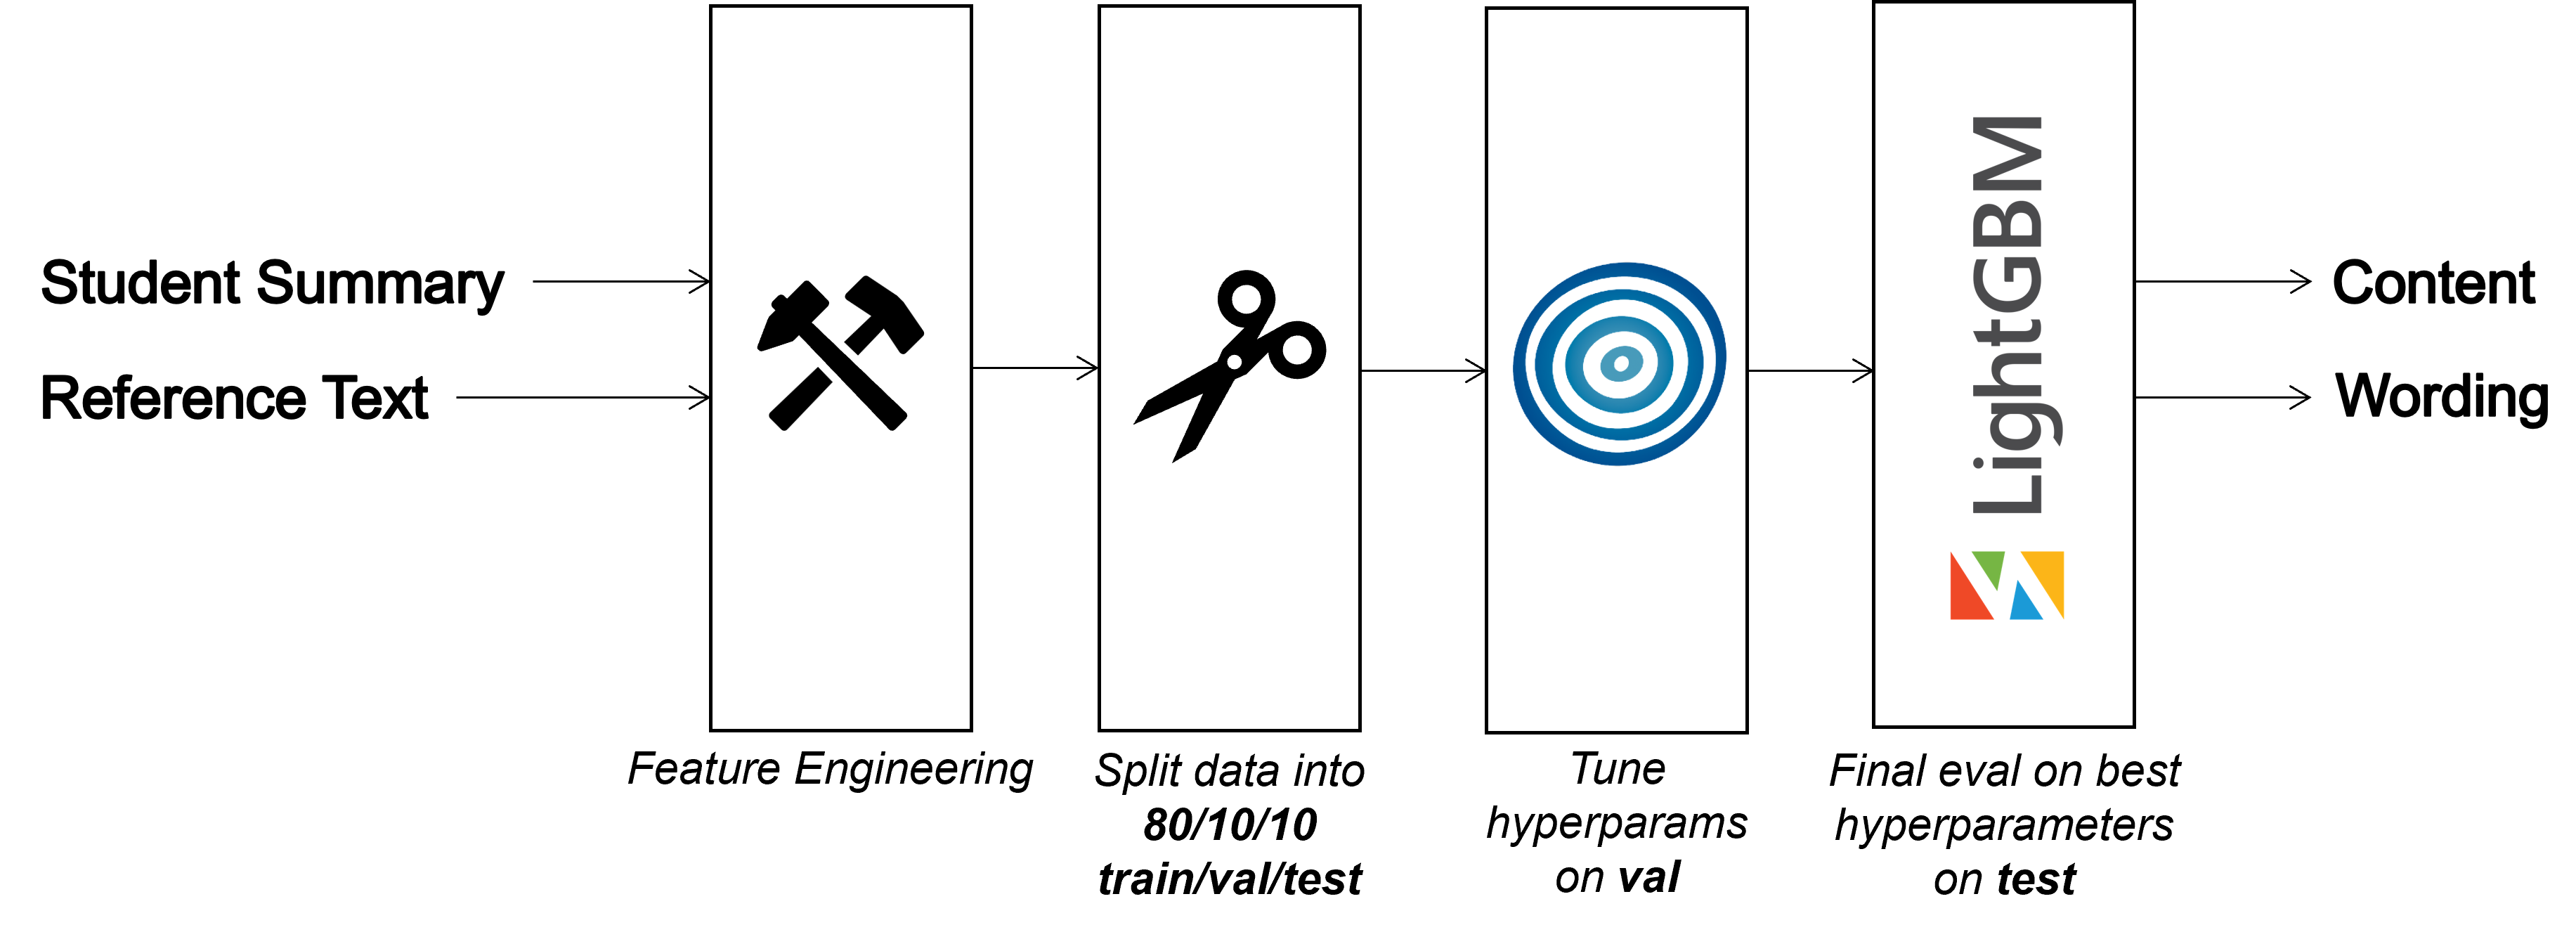
\includegraphics[keepaspectratio, width=\textwidth]{img/lightgbm-architecture.png}
\caption[Pipeline of the LightGBM Model]{Pipeline of the LightGBM model, the feature engineering was done using the aforementioned Textstat library and the hyperparameters were tuned with the help of Optuna}
\label{fig:lightgbm-model}
\end{figure}

\subsubsection{Hyperparameters}

For the LightGBM model, Optuna was used. Optuna allows for efficient hyperparameter tuning by optimizing an objective function. Additional details can be found by referring to the original article under \cite{10.1145/3292500.3330701}.\\

\noindent These are the final hyperparameters that have been used for this model:

\begin{itemize}
	\item \textbf{Number of Estimators
:} 778
	\item \textbf{Learning Rate
:} 0.015
	\item \textbf{Colsample Bytree
:} 0.761
	\item \textbf{Reg Alpha
:} 0.002
\end{itemize}

\noindent Those final hyperparameters have been used after using Optuna to determine the importance of every hyperparameter and only using those four, which had the highest importance. This was done to maximize the hyperparameter search speed for any subsequent training. Any definitions can be found in the glossary.

\subsubsection{Results}

The final \gls{mcrmse} scores of the LightGBM model were as follows:

\begin{itemize}
	\item \textbf{Content RMSE:} 0.66
	\item \textbf{Wording RMSE:} 0.51
	\item \textbf{MCRMSE:} 0.59
\end{itemize}

\noindent This model performs better on the wording score than the other approaches in this project. This was one of the reasons for choosing an ensemble-based approach to improve the final score.
